%---------------------------------------------------------------------
% Chapter 7: Observability and Evaluation
% Numbers: \res{...} macros from ../generated/results.tex (run 2, seed 7); the few hand-typed
% values (reasoning p95, Phoenix span times, error counts) are sourced in FACTS.md sections 12 and 23.
%---------------------------------------------------------------------
\chapter{Observability and Evaluation}
\label{ch:eval}

This chapter describes how a check is made visible while it runs and how the agent was measured
against a simpler lookup. All numbers come from our own runs. Evaluation numbers come from
\texttt{paper/generated/results.tex}, written by \texttt{cli.py eval}; the few values typed by hand
(the reasoning 95th percentile, the Phoenix span times and the error counts) are taken from
\texttt{docs/results/eval\_seed7.md} and \texttt{docs/trace/} and listed in \texttt{FACTS.md}. The reported run is the second run on the evaluation seed; the first run and the
code changes between the two are disclosed in Chapter~\ref{ch:exp}.

\section{Tracing and Monitoring}
\label{sec:eval-tracing-and-monitoring}

\begingroup\setlength{\emergencystretch}{3em}
\paragraph{JSONL step log.} Every check writes one JSON-lines file, named
\texttt{data/\allowbreak traces/\allowbreak <thread\_id>.jsonl}, which the API serves at \texttt{GET /api/traces/<id>}.
Each line carries the UTC time, the check identifier and the event name. Step events add the step
number, the action, the planner source (\texttt{rules}, \texttt{llm}, \texttt{rules(fallback)},
\texttt{rules(verifier)} or \texttt{user}), a one-line summary and the duration in milliseconds, and,
where present, the planner's thought, the learned prior and the verifier result (event list in
Section~\ref{sec:concepts-observability}). The schema has fields for the model name and token
counts that the current code does not fill, so token usage is not reported; the model name and the
duration of each model call are recorded in the OpenTelemetry span described next. Cost is zero by
construction, because the only model is a local one. A failure in the tracer is swallowed, so
writing a trace can never fail a check. The same events stream to the client over server-sent
events and drive its live step timeline.\par\endgroup

\paragraph{OpenTelemetry and Phoenix.} When \texttt{STRIPCHECK\_TRACING=1} is set, the same check
is exported as OpenTelemetry spans to a local Arize Phoenix server (version 21.0.0) using the
OpenInference conventions~\cite{otel2026genai,arize2026openinference}. A 0.25\,s TCP probe, cached
for 15\,s, skips span creation when Phoenix is not running, and the exporter has a 3\,s timeout.
Each check becomes one trace: a root \texttt{check} span (\textsc{agent}), a
\texttt{planner:~<action>} span per step (\textsc{chain}) with its \textsc{tool} span, a
\texttt{planner\_llm} span (\textsc{llm}) at each model consultation, a \texttt{verifier} span
(\textsc{guardrail}), and a \texttt{check.resume} span for the half after an answer.

Figure~\ref{fig:phoenix-trace} shows the span tree of the misread walkthrough of
Section~\ref{sec:design-data-flow} (25 spans). In the exported spans (\texttt{docs/trace/phoenix\_spans\_run1.json}) the two
\texttt{planner\_llm} spans took 4.60\,s and 3.89\,s of the 8.49\,s root span, and every tool span
took under a millisecond, so the model calls account for almost all of the time. Phoenix shows
these durations truncated to one decimal (4.5\,s, 3.8\,s and 8.4\,s), and the 8.8\,s in its header is
the trace latency that Phoenix measures for the whole trace, including the resumed half. The root
span's input and output are shown in Figure~\ref{fig:app-phoenix-io} of Appendix~\ref{app:traces}.
With Ollama unreachable, the same check finished in about 2\,s with \texttt{rules(fallback)} at both
branch points and the same \FLAGGED{} result (\texttt{docs/trace/README.md}), which is the behaviour
the fallback is designed for.

\begin{figure}[htbp]
\centering
\begin{tikzpicture}
\node[anchor=south west,inner sep=0] (img) at (0,0)
  {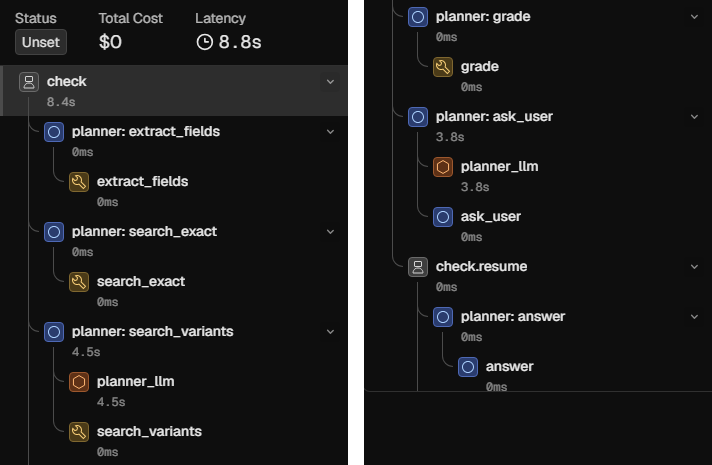
\includegraphics[width=\linewidth]{fig_phoenix_tree.png}};
\begin{scope}[x={(img.south east)},y={(img.north west)},
  callout/.style={circle,fill=BrickRed,text=white,font=\bfseries\footnotesize,inner sep=1.2pt,minimum size=13pt}]
  \node[callout] at (0.405,0.914) {1};  % trace latency and cost
  \node[callout] at (0.160,0.824) {2};  % root check span (agent)
  \node[callout] at (0.285,0.166) {3};  % planner_llm before search_variants
  \node[callout] at (0.805,0.630) {4};  % planner_llm before ask_user
  \node[callout] at (0.775,0.424) {5};  % check.resume
\end{scope}
\end{tikzpicture}
\caption{Span tree of the Review~3 misread walkthrough in Phoenix (synthetic pack, hybrid planner),
cropped and split into two columns; the right column continues the left one. (1)~trace latency
8.8\,s and cost \$0 (local model); (2)~root \texttt{check} span of kind \textsc{agent} (8.49\,s,
shown truncated as 8.4\,s); (3)~branch point after the empty exact search, where the model chose
\texttt{search\_variants} (4.60\,s); (4)~branch point after grading, where the model chose
\texttt{ask\_user} (3.89\,s); (5)~the resumed half of the check under the same root.}
\label{fig:phoenix-trace}
\end{figure}

\paragraph{Monitoring.} The evaluation harness counts steps by planner source (model or fallback),
and \texttt{cli.py doctor} reports the database counts, the installed readers and whether Ollama
and Phoenix are reachable.

\section{Evaluation Dataset}
\label{sec:eval-evaluation-dataset}

Eleven authored diagnostic scenarios check behaviour in the test suite and are not used as an
accuracy measure. The evaluation uses the golden set generated by \texttt{cli.py props --eval}, which renders
\res{ResN} cartons from real alert rows of the local index of \res{ResAlertCount} alerts, and every
image carries the banner ``DEMO PROP - NOT A MEDICINE''. No team member labels the packs by hand:
the generator writes the truth label and the printed fields of each pack to a manifest when it
renders the carton, so labels are correct by construction. Clean, glare, QR, misread and spurious
packs carry a listed batch (40 packs); not-listed controls carry an invented batch, collisions a
listed batch number on a different product and maker, and siblings an unlisted batch one look-alike
character from a listed one (20 packs). Table~\ref{tab:eval-mix} in Appendix~\ref{app:supp} gives
the count and truth label of each scenario. Two seeds
of the generator give two disjoint sets of packs. Seed~1 is the development set, on which the
thresholds were tuned, and seed~\res{ResSeed} is the evaluation set reported here. Misread and
sibling packs print the misread string on the carton, so the OCR error is simulated, and the oracle
user answers from the batch the pack was meant to carry (decision D24). Perception is shared by all
arms and runs once per image: the reader (RapidOCR PP-OCRv6-small) returned the rendered batch on
\res{ResOCRBatchExact} images of seed~\res{ResSeed}, at a median of \res{ResOCRMedian}\,s per image.

\section{Metrics and Evaluation Rubric}
\label{sec:eval-metrics-and-evaluation-rubric}

Let $P$ be the packs whose truth is \FLAGGED{} or \SFAKE{}, $N$ the packs whose truth is \NLISTED{},
$A=\{\FLAGGED,\SFAKE\}$ the alarm labels and $\hat{y}_i$ the label an arm returns for pack $i$. The
metrics are defined as in \texttt{core/evaluate.py}:
\begin{align*}
\text{hit recall} &= \frac{|\{i\in P:\hat{y}_i\in A\}|}{|P|}, &
\text{type accuracy} &= \frac{|\{i\in P:\hat{y}_i=y_i\}|}{|\{i\in P:\hat{y}_i\in A\}|},\\[2pt]
\text{false-alarm rate} &= \frac{|\{i\in N:\hat{y}_i\in A\}|}{|N|}, &
\text{abstention rate} &= \frac{|\{i:\hat{y}_i=\CANTV\}|}{n}.
\end{align*}
The false-alarm rate is also reported on the collision and sibling packs alone. Overall accuracy is
the share of all packs whose label equals the truth. Questions per pack and steps per pack are
averages over all packs. Latency per pack is the shared perception time plus the arm's own reasoning
time; we report the median, the mean and the 95th percentile (linear interpolation). A safety
violation is a banned phrase in the headline, explanation or advice, an unknown label, or an alarm
without a citation, and the required count is zero.

Rates carry 95\% Wilson score intervals~\cite{wilson1927probable,brown2001interval}, which stay
inside $[0,1]$ and behave well at $k=0$ and $k=n$, where most of our cells lie. Paired comparisons
on the same packs use the exact two-sided McNemar test~\cite{mcnemar1947note,dietterich1998approximate}
on per-pack correctness, $p=\min\bigl(1,\,2\sum_{i=0}^{\min(b,c)}\binom{b+c}{i}2^{-(b+c)}\bigr)$,
where $b$ counts packs only the agent gets right and $c$ packs only the baseline gets right. With at
most eight packs per scenario, per-scenario results are given as counts.

No language model judges the output: the verdict is one of four discrete labels and the truth is
fixed by the manifest, so each pack is scored by exact comparison.

\section{Baselines}
\label{sec:eval-baselines}

Arm~A, the baseline, is a lookup script that does what a person can do with the CDSCO list viewer:
it takes the batch from the QR code or OCR, normalises it, looks it up exactly in the index and
reports any hit as an alarm (\SFAKE{} for a spurious entry, \FLAGGED{} otherwise). It uses the same
perception output, the same index of \res{ResAlertCount} alerts and the same verdict templates as
the agent, so the arms differ only in the reasoning between the read batch and the verdict. Arm~B is the agent with the rule planner and arm~C the agent with the
hybrid planner, which consults \texttt{qwen2.5:3b} through Ollama at the two branch points
(temperature~0). Each arm runs under two human-in-the-loop policies: an \emph{oracle} user who
answers every question truthfully from the manifest, and \emph{none}, where every question is
skipped. The second policy acts as an ablation of the human loop.

\section{Results}
\label{sec:eval-results}

Table~\ref{tab:eval-results} gives the headline metrics for the three arms under both policies.

\begin{table}[htbp]
\centering
\caption[Headline metrics on the evaluation set (seed~7, run~2)]{Headline metrics on the evaluation set (seed~7, $n=60$, run~2). Rates as value ($k/n$) with
the Wilson 95\% interval below. Source: \texttt{paper/generated/results.tex}.}
\label{tab:eval-results}
\footnotesize
\setlength{\tabcolsep}{4pt}
\renewcommand{\arraystretch}{1.12}
\begin{tabularx}{\linewidth}{@{}>{\raggedright\arraybackslash}X ccc@{}}
\toprule
\textbf{Metric} & \textbf{Baseline (lookup)} & \textbf{Agent (rules)} & \textbf{Agent (hybrid)} \\
\midrule
\multicolumn{4}{@{}l}{\textit{HITL = oracle (a person answers every question)}} \\
Hit recall & \res{ResBaseOracleHitRecall} (\res{ResBaseOracleHitRecallK}) & \res{ResRulesOracleHitRecall} (\res{ResRulesOracleHitRecallK}) & \res{ResHybridOracleHitRecall} (\res{ResHybridOracleHitRecallK}) \\
 & \res{ResBaseOracleHitRecallCI} & \res{ResRulesOracleHitRecallCI} & \res{ResHybridOracleHitRecallCI} \\
Hit recall, clean and QR & \res{ResBaseOracleHitRecallCleanQR} (\res{ResBaseOracleHitRecallCleanQRK}) & \res{ResRulesOracleHitRecallCleanQR} (\res{ResRulesOracleHitRecallCleanQRK}) & \res{ResHybridOracleHitRecallCleanQR} (\res{ResHybridOracleHitRecallCleanQRK}) \\
Type accuracy & \res{ResBaseOracleTypeAcc} (\res{ResBaseOracleTypeAccK}) & \res{ResRulesOracleTypeAcc} (\res{ResRulesOracleTypeAccK}) & \res{ResHybridOracleTypeAcc} (\res{ResHybridOracleTypeAccK}) \\
False-alarm rate, all not listed & \res{ResBaseOracleFAR} (\res{ResBaseOracleFARK}) & \res{ResRulesOracleFAR} (\res{ResRulesOracleFARK}) & \res{ResHybridOracleFAR} (\res{ResHybridOracleFARK}) \\
 & \res{ResBaseOracleFARCI} & \res{ResRulesOracleFARCI} & \res{ResHybridOracleFARCI} \\
False-alarm rate, collisions & \res{ResBaseOracleFARCollision} (\res{ResBaseOracleFARCollisionK}) & \res{ResRulesOracleFARCollision} (\res{ResRulesOracleFARCollisionK}) & \res{ResHybridOracleFARCollision} (\res{ResHybridOracleFARCollisionK}) \\
False-alarm rate, siblings & \res{ResBaseOracleFARSibling} (\res{ResBaseOracleFARSiblingK}) & \res{ResRulesOracleFARSibling} (\res{ResRulesOracleFARSiblingK}) & \res{ResHybridOracleFARSibling} (\res{ResHybridOracleFARSiblingK}) \\
Abstention rate & \res{ResBaseOracleAbstain} (\res{ResBaseOracleAbstainK}) & \res{ResRulesOracleAbstain} (\res{ResRulesOracleAbstainK}) & \res{ResHybridOracleAbstain} (\res{ResHybridOracleAbstainK}) \\
Overall accuracy & \res{ResBaseOracleAccuracy} (\res{ResBaseOracleAccuracyK}) & \res{ResRulesOracleAccuracy} (\res{ResRulesOracleAccuracyK}) & \res{ResHybridOracleAccuracy} (\res{ResHybridOracleAccuracyK}) \\
 & \res{ResBaseOracleAccuracyCI} & \res{ResRulesOracleAccuracyCI} & \res{ResHybridOracleAccuracyCI} \\
Questions / steps per pack & \res{ResBaseOracleQuestions} / \res{ResBaseOracleSteps} & \res{ResRulesOracleQuestions} / \res{ResRulesOracleSteps} & \res{ResHybridOracleQuestions} / \res{ResHybridOracleSteps} \\
Latency median / mean / p95 (s) & \res{ResBaseOracleLatMedian} / \res{ResBaseOracleLatMean} / \res{ResBaseOracleLatPNinetyFive} & \res{ResRulesOracleLatMedian} / \res{ResRulesOracleLatMean} / \res{ResRulesOracleLatPNinetyFive} & \res{ResHybridOracleLatMedian} / \res{ResHybridOracleLatMean} / \res{ResHybridOracleLatPNinetyFive} \\
LLM steps / fallback steps & \res{ResBaseOracleLLMSteps} / \res{ResBaseOracleFallbackSteps} & \res{ResRulesOracleLLMSteps} / \res{ResRulesOracleFallbackSteps} & \res{ResHybridOracleLLMSteps} / \res{ResHybridOracleFallbackSteps} \\
Safety violations & \res{ResBaseOracleSafety} & \res{ResRulesOracleSafety} & \res{ResHybridOracleSafety} \\
\midrule
\multicolumn{4}{@{}l}{\textit{HITL = none (every question skipped)}} \\
Hit recall & \res{ResBaseSkipHitRecall} (\res{ResBaseSkipHitRecallK}) & \res{ResRulesSkipHitRecall} (\res{ResRulesSkipHitRecallK}) & \res{ResHybridSkipHitRecall} (\res{ResHybridSkipHitRecallK}) \\
 & \res{ResBaseSkipHitRecallCI} & \res{ResRulesSkipHitRecallCI} & \res{ResHybridSkipHitRecallCI} \\
Hit recall, clean and QR & \res{ResBaseSkipHitRecallCleanQR} (\res{ResBaseSkipHitRecallCleanQRK}) & \res{ResRulesSkipHitRecallCleanQR} (\res{ResRulesSkipHitRecallCleanQRK}) & \res{ResHybridSkipHitRecallCleanQR} (\res{ResHybridSkipHitRecallCleanQRK}) \\
False-alarm rate, all not listed & \res{ResBaseSkipFAR} (\res{ResBaseSkipFARK}) & \res{ResRulesSkipFAR} (\res{ResRulesSkipFARK}) & \res{ResHybridSkipFAR} (\res{ResHybridSkipFARK}) \\
Abstention rate & \res{ResBaseSkipAbstain} (\res{ResBaseSkipAbstainK}) & \res{ResRulesSkipAbstain} (\res{ResRulesSkipAbstainK}) & \res{ResHybridSkipAbstain} (\res{ResHybridSkipAbstainK}) \\
Overall accuracy & \res{ResBaseSkipAccuracy} (\res{ResBaseSkipAccuracyK}) & \res{ResRulesSkipAccuracy} (\res{ResRulesSkipAccuracyK}) & \res{ResHybridSkipAccuracy} (\res{ResHybridSkipAccuracyK}) \\
Safety violations & \res{ResBaseSkipSafety} & \res{ResRulesSkipSafety} & \res{ResHybridSkipSafety} \\
\bottomrule
\end{tabularx}
\end{table}


With the oracle user both agent arms raised an alarm on all \res{ResRulesOracleHitRecallK} listed
packs and on none of the \res{ResRulesOracleFARK} not-listed packs. The lookup missed the eight
misread packs and raised an alarm on all eight collisions and all four siblings, so its false-alarm
rate on not-listed packs was \res{ResBaseOracleFAR} (\res{ResBaseOracleFARK}). On the clean, QR and
spurious packs the two approaches agree. Figure~\ref{fig:eval-scenarios} breaks the result down by
scenario and shows that the baseline fails exactly where a batch number alone is misleading.

\begin{figure}[htbp]
\centering
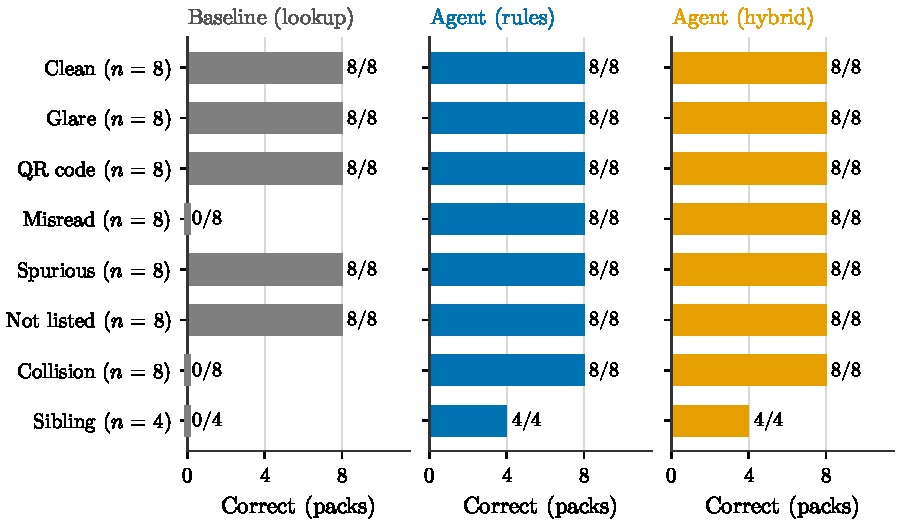
\includegraphics{fig_scenarios_seed7.pdf}
\caption{Correct verdicts per scenario on seed~7 with a person answering ($n=8$ per scenario, 4 for
siblings). ``Not listed'' denotes the not-listed control packs. The baseline fails on the misread,
collision and sibling packs.}
\label{fig:eval-scenarios}
\end{figure}

The agent's advantage depends on the person. When every question is skipped
(Figure~\ref{fig:eval-hitl} in Appendix~\ref{app:supp}), hit recall falls to \res{ResRulesSkipHitRecall}
(\res{ResRulesSkipHitRecallK}) and the agent abstains on \res{ResRulesSkipAbstainK} packs, which is
lower accuracy than the lookup (\res{ResRulesSkipAccuracyK} against \res{ResBaseSkipAccuracyK}). The
false-alarm rate stays at \res{ResRulesSkipFAR}, because rule R2 never turns an unconfirmed
machine read into an alarm. The packs it still gets right without answers are the QR packs, whose
batch is confirmed by the code, and the collision and not-listed control packs, which end in
\NLISTED{} without a question.

Figure~\ref{fig:eval-latency} (Appendix~\ref{app:supp}) gives the cost. Perception dominates every arm: the median end-to-end
time was \res{ResBaseOracleLatMedian}\,s for the lookup and \res{ResRulesOracleLatMedian}\,s for the
rule agent, whose reasoning took a median of \res{ResRulesOracleReasonMedian}\,s (95th percentile
0.103\,s). The hybrid planner had \res{ResHybridOracleFallbackSteps} fallbacks to rules. Its median rose only to
\res{ResHybridOracleLatMedian}\,s, because the model is consulted only at branch points
(\res{ResHybridOracleLLMSteps} times over \res{ResN} packs), but each model call
takes seconds on the laptop, so its 95th percentile was \res{ResHybridOracleLatPNinetyFive}\,s.
No arm produced a safety violation.

\section{Error Analysis}
\label{sec:eval-error-analysis}

Table~\ref{tab:eval-errors} groups every incorrect verdict of run~2 on seed~7, taken from the
per-pack listing in \texttt{docs/results/eval\_seed7.md}. Examples are schematic, because the packs
carry batch strings from CDSCO rows. With the oracle user the two agent arms
made no error, so the table lists the baseline's 20 errors and the agent's 36 abstentions when
questions are skipped. The seven alarms the agent missed in run~1, before the fixes, are analysed
in Section~\ref{sec:exp-results}.

\begin{table}[htbp]
\centering
\caption{Incorrect verdicts on seed~7 (run~2) grouped by cause, with one example per group}
\label{tab:eval-errors}
\small
\begin{tabularx}{\linewidth}{@{}>{\raggedright\arraybackslash}p{0.21\linewidth} c
  >{\raggedright\arraybackslash}X >{\raggedright\arraybackslash}p{0.25\linewidth}@{}}
\toprule
\textbf{Arm and cause} & \textbf{Count} & \textbf{Example} & \textbf{What addresses it} \\
\midrule
Baseline: misread batch not found & 8 & A listed \texttt{Z} printed as \texttt{2} (schematic:
listed \texttt{AZ1234}, carton \texttt{A21234}); lookup returns \NLISTED & Confusion-aware variant search with a person
confirming the character (agent) \\
Baseline: collision raised as alarm & 8 & Listed batch number on a different product and maker;
lookup returns \FLAGGED & Grading of product, dates and maker before any alarm (agent) \\
Baseline: sibling raised as alarm & 4 & Carton reads a listed batch one look-alike character
away from the unlisted batch the pack carries (schematic: \texttt{AB1703} read, \texttt{AB1708}
carried); lookup returns \FLAGGED & Batch confirmation by the person before an
alarm (agent) \\
Agent, no answers: batch gate & 28 & Clean, glare, spurious and sibling packs whose
\texttt{confirm\_batch} question was skipped end in \CANTV & A QR code or a second photo as
independent evidence; otherwise only the person \\
Agent, no answers: character unconfirmed & 8 & Misread packs whose \texttt{confirm\_char} question
was skipped end in \CANTV & Only the person holding the pack \\
\bottomrule
\end{tabularx}
\end{table}

The baseline's errors are structural. A lookup cannot recover a batch that the reader got wrong, and
it cannot tell whether a listed batch number belongs to this product, so collisions and siblings
become false alarms. The test set over-represents these traps by design, so this false-alarm rate
is not an estimate of the rate in use (Section~\ref{sec:lim-limitations}).
The agent's 36 abstentions are the designed behaviour of the batch gate; their cost is recall
without a human, which only stronger independent evidence (a QR code on more packs, or a second
agreeing read) can reduce. These results show that the reasoning behaves as designed on rendered traps; they do not
measure accuracy on photographs of real strips (Chapter~\ref{ch:lim}).
